\section{Introdução} 
\frame{\tableofcontents[currentsection]}

\subsection{O que é?} % A subsection can be created just before a set of slides with a common theme to further break down your presentation into chunks

%-----------------------------------------------
\begin{frame}
	\frametitle{Definição}

	\Large{\azul{\textbf{Expressão Regular}} é:}

	\begin{itemize}
		\item Uma "linguagem de programação"\cite{hopcroft};
		\item Intimamente relacionada aos \azul{DFA}, que são \textit{\azul{autômatos}}, analisadores sintáticos\cite{hopcroft};
		\item Uma maneira sucinta e \azul{finita} de representar uma linguagem infinita - regular;
		\item É um método formal de se especificar um padrão de texto\cite{aurelio}.
	\end{itemize}

\end{frame}

%------------------------------------------------
\begin{frame}
	\begin{block}{Mesmo, Eu.}
	"Uma imagem vale mais do que mil palavras. Uma Expressão Regular\footnote{bombeável} vale infinitas."
	\end{block}
\end{frame}
%------------------------------------------------

\begin{frame}
	\frametitle{Observação importante:}
	\centering \Large{Diferença da teoria e da prática.}
\end{frame}

%------------------------------------------------
\subsection{Parte prática!}

\begin{frame}
	\Large{\azul{\textbf{Vamos deixar claro nosso escopo!}}}
\end{frame}

%------------------------------------------------
\begin{frame}
	\frametitle{Para a felicidade de alguns, infelicidade de outros...}
	
	\begin{itemize}
		\item Nosso escopo nessa apresentação é mais \azul{prático} e não teórico;
		\item Vamos aprender \azul{como} usar;
		\item Vamos aprender \azul{onde} usar;
		\item Vamos aprender \azul{porque} usar.
	\end{itemize}
\end{frame}

\subsection{Você não vai aprender isso nessa apresentação!}

%------------------------------------------------
\begin{frame}
\frametitle{Nada de lógica}
\centering
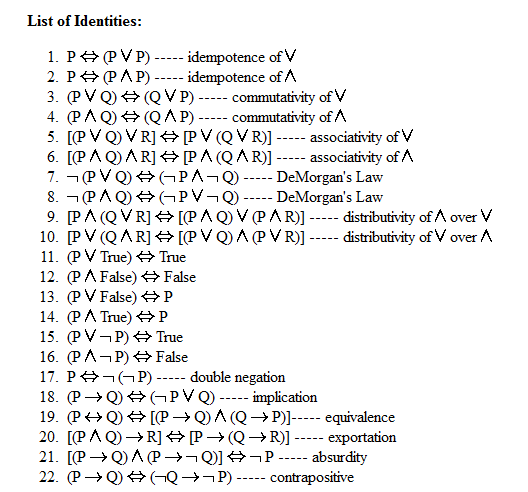
\includegraphics[width=0.8\textwidth]{./imagens/re/logica.png}
\end{frame}
%------------------------------------------------
\begin{frame}
\frametitle{Nada de transição de DFA para NFA}
\centering
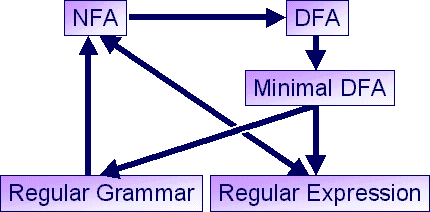
\includegraphics[width=0.8\textwidth]{./imagens/re/NFA-DFA.png}
\end{frame}
%------------------------------------------------
\begin{frame}
\frametitle{Não vamos aprender autômatos}
\centering
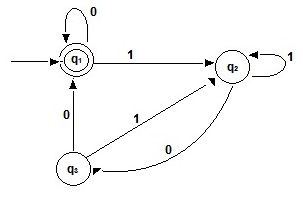
\includegraphics[width=0.8\textwidth]{./imagens/re/NFA.jpg}
\end{frame}
%------------------------------------------------

\subsection{Você vai aprender muito isso!}
%------------------------------------------------
\begin{frame}
\frametitle{Isso vai fazer parte da sua realidade}
\centering
\bf
\Large{\textasciicircum *[A-Za-z0-9\_]+:(.*)\$}
\end{frame}
%------------------------------------------------
\begin{frame}
\frametitle{Isso não vai te dar mais pânico!}
\centering
\bf
\Large{([0-9]\{1,3\}\textbackslash.)\{2\}[0-9]\{1,3\}-[0-9]\{2\}}
\end{frame}
%------------------------------------------------
\begin{frame}
\frametitle{Isso será fácil de entender (:}
\centering
\bf
\Large{[-+]?[0-9]\{1,3\}(\textbackslash.[0-9]\{3\})?(,[0-9]\{2\})?}
\end{frame}
%------------------------------------------------
\begin{frame}
\begin{figure}
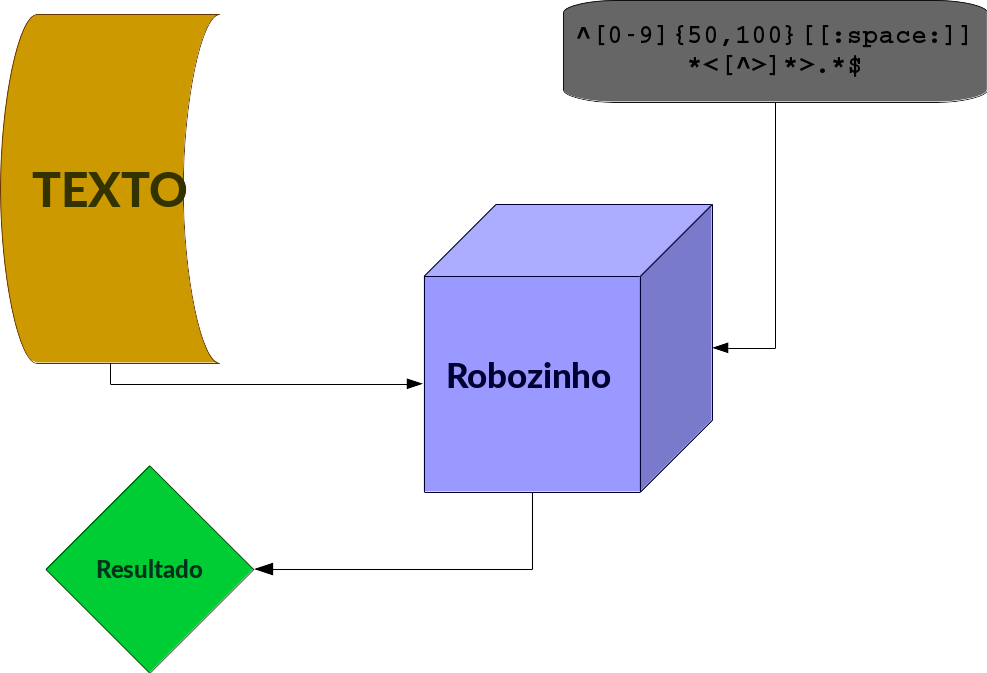
\includegraphics[height=0.75\textheight]{./imagens/re/como-vai-funcionar.png}
\caption{Como vamos abordar as RE}
\end{figure}
\end{frame}

\subsection{Livro}

\begin{frame}
\frametitle{[Expressões Regulares] Uma abordagem divertida}

\begin{figure}[h]
\centering

\includegraphics[height=0.75\textheight]{./imagens/re/piazinho.jpg}
\caption{Essa apresentação foi \azul{inspirada}, \azul{causada} e \azul{é} sobre esse livro.}
\end{figure}
\end{frame}

